\chapter{Asking Entrepreneurs How They Got Rich (San Antonio)}

We begin with an Audi R8 teaser and two large income claims, and only then does the lecture ask its real question: what machinery sits underneath those numbers, and what can a younger viewer do with it now? There is no surviving board here to settle notation for us, so whenever we write an equation we are making the mildest possible transcript-backed reconstruction. The lecture itself moves from observable results to operating rules: staged growth, reputation, perseverance, land, long-horizon craft, then a layered business model linking real estate, Airbnb, Turo, and exotic cars.

\section{Opening Setup: Observable Scale Before Explanation}

The opening montage is deliberately front-loaded with magnitude. We are shown outcomes first, because the lecture wants credibility before theory. A million-dollar year, more than half a million dollars, and later a net worth in the range of \$15\text{M}--\$20\text{M}: these numbers are not yet the lesson, but they establish that the later rules are being extracted from real operating experience.

\begin{align}
G_{\text{peak}}^{(1)} &\approx \$1{,}000{,}000,\\
G_{\text{peak}}^{(2)} &> \$500{,}000,\\
W_{\text{developer}} &\approx \$15\text{M}-\$20\text{M}.
\end{align}

We should pause over the order. The lecture does not begin by saying what wealth is in general. It begins by saying, in effect: here are people who have actually touched scale; now let us ask what repeated structure made that possible.

\paragraph{Claim.} Wealth first appears as a set of reported observables: annual gross, portfolio size, net worth, and fleet size.

\paragraph{Mechanism.} The chapter should therefore move, as the lecture moves, from credential to causal rule. Each time, we ask not merely what happened, but what was done repeatedly enough to make it happen.

\section{Crawl, Walk, Run: Scale and Recoverability}

The first substantial interview belongs to an operator who has moved across wealth management, company leadership, and construction. The lecture uses this breadth to introduce its first strict rule of order: growth should be staged, because leverage without expertise is not scale but fragility.

We may compress the rule into the form
\begin{equation}
\text{crawl} \to \text{walk} \to \text{run},
\qquad
\text{expertise} \prec \text{leverage}.
\end{equation}

The point is not that caution is always superior to speed. The point is that speed only becomes useful after the operator knows enough to recover from error. The speaker says this plainly: if we run too fast, we may over-leverage; if we over-leverage before we know the business, then a small mistake becomes a capital event.

\subsection{Question \& Answer}

\paragraph{Question.} How do we scale without destroying ourselves?

\paragraph{Answer.} We scale in an order that preserves recoverability. We learn the business first, become expert in it, and only then tolerate the larger exposures that come with faster growth.

\paragraph{Mechanism.} What matters is not speed in isolation but the ability to stand back up after a mistake. The lecture's first principle is therefore not merely \emph{grow}; it is \emph{grow in a way that leaves learning possible after failure}.

The section then makes a move that is easy to flatten if we are careless. Asked for the best financial decision of his career, the speaker points to marriage and a good personal life. The lecture is not drifting off topic. It is broadening the variable list. Stability at home is treated as part of the operating environment of disciplined business action.

\section{Reputation, Friction, and the AI Pivot}

The first operator leaves us with another maxim: every day is an interview, every day is a resume. The lecture is still talking about wealth, but it has now shifted from balance-sheet structure to repeated conduct. What matters is not the thirty-minute formal interaction alone, but the total pattern of attitude, behavior, and reliability.

At this point the lecture inserts a caricature intermission. The pause is not filler. It resets the pace and gives the episode a running clock. When we return, we meet a bioinformatics founder who has just sold a business. Again the sequence is the same: industry, outcome, advice. The lesson this time is perseverance.

The key claim is that friction is not accidental noise around the path of growth. It is part of the medium through which growth is obtained. The transcript is clear on this point: everybody experiences friction, and the people who make it are the ones who continue anyway.

\subsection{Question \& Answer}

\paragraph{Question.} What separates the founder who survives early adversity from the one who exits too soon?

\paragraph{Answer.} The lecture gives a two-part answer. First, we continue through friction rather than reading friction itself as a final verdict. Second, we remain adaptive enough to update our tool set while doing so.

That second point becomes the explicit AI pivot. The transcript's claim is not that AI replaces work in the abstract. It is that a worker who knows how to use AI may replace one who does not. The lecture thus shifts the problem from science fiction to comparative capability.

\begin{remark}
The transcript's phrasing around ``chat, chat, GTP'' is noisy, but the intended reference is clearly to ChatGPT and related tools. The conceptual point is stable even if the transcript is imperfect.
\end{remark}

\section{Westin Pivot: Land, Carrying Cost, and Risk}

The lecture now announces a spatial transition: the Riverwalk interviews are wrapped, and we move into the Westin. This reset matters because the topic sharpens. We are no longer asking merely about entrepreneurship in general; we are asking where new money should go if one wants to multiply it.

The developer's answer is land. The logic is given in pieces, and we should preserve those pieces rather than replacing them with abstract real-estate prose. First, nobody is making more land. Second, development costs rise. Third, the land can be held under favorable conditions if it has agricultural use. Fourth, the upside appears later, at sale or development.

A compact reconstruction of the mechanism is
\begin{equation}
\text{fixed supply of land} + \text{rising development cost}
\;\Longrightarrow\;
\text{scarcity value with development optionality}.
\end{equation}

The lecture also gives us a structural statement about the burden of holding:
\begin{equation}
\text{carry cost} = \text{tax burden} + \text{other holding costs},
\qquad
\text{agricultural use} \Rightarrow \text{smaller tax burden}.
\end{equation}

No tax rates are supplied, and so we do not invent them. The claim is qualitative but economically precise: a lighter carrying burden buys time, and time preserves optionality.

\subsection{Question \& Answer}

\paragraph{Question.} Why land, and why take the plunge instead of waiting for certainty?

\paragraph{Answer.} Land is attractive here because scarcity and development cost growth push in the same direction. Risk is justified because even failure generates information. The lecture does not celebrate reckless exposure; it celebrates exposure that teaches.

\paragraph{Mechanism.} The hidden asset is not land alone, but land plus time plus the option to act later.

\section{Return to the Riverwalk: Long-Horizon Craft and Lifestyle}

The lecture returns to the caricature artist, and once again the pacing changes. We are no longer in the language of net worth and development optionality. We are in the language of long-horizon practice. The artist reports roughly \(35\) years of work, a continuing affection for the public, and a cumulative output that is striking enough to deserve a quantitative pause:
\begin{equation}
N_{\text{drawn}} \approx 5\times 10^5.
\end{equation}

A careful average-rate estimate shows the scale of this repetition:
\begin{align}
T &\approx 35\ \text{years},\\
\bar N_{\text{year}} &\approx \frac{N_{\text{drawn}}}{T}
\approx \frac{500{,}000}{35}
\approx 1.43\times 10^4\ \text{drawings per year}.
\end{align}

This is not an assertion of uniform output. It is simply a way of making visible what decades of practice look like once accumulated. The artist's advice to the younger generation is then a direct verbalization of the same arithmetic: believe in yourself, do not give up, keep moving, and the large total eventually appears.

The architect interview that follows deepens the same point from another angle. Here the income range is smaller,
\begin{equation}
G_{\text{architect}} \approx \$300{,}000-\$400{,}000 \text{ per year},
\end{equation}
but the advice is economically serious: choose according to the lifestyle one wants to live. The lecture is insisting that the optimization problem is not one-dimensional. Higher income is one coordinate, but the shape of life remains part of the solution.

\subsection{Question \& Answer}

\paragraph{Question.} What does persistence buy us, if not the exact form of early fame we imagined?

\paragraph{Answer.} In this lecture it buys cumulative output, competence, credibility, and a sustainable place in the world. The fantasy may change; the compounding need not.

\section{From Passion to the First Deal}

Only now does the lecture cash in the R8 teaser. The owner is no longer a visual hook but a full case study. The first advice is consistency, then discipline, then real-estate entry. The transcript reports approximately \$1.3M gross at peak, though the phrasing is colloquial enough that we should write it with care:
\begin{equation}
G_{\text{peak,R8 owner}} \approx \$1.3\text{M}.
\end{equation}

The lecture's next move is very characteristic. It does not tell us to chase random opportunities. It says to begin with something one is passionate enough about to study deeply, then to invest in it, learn everything around it, and duplicate the deal structure. In the lecture's own logic, the path is
\begin{equation}
\text{research} \to \text{first deal} \to \text{duplication at scale}.
\end{equation}

We are told that the operator now has roughly
\begin{equation}
N_{\text{properties}} \approx 38-40.
\end{equation}
Humility then appears as a control variable. Staying humble keeps learning open, and an open learner is harder to trap inside early success.

\subsection{Question \& Answer}

\paragraph{Question.} If we have zero properties and zero rentals, what is the first step?

\paragraph{Answer.} Research, and research in an order. We examine the city, then the exact area, then the platform itself. Only after that do we try to control a unit and test the offer.

\paragraph{Worked example.} The lecture gives a gross monthly range for a first property. We can annualize it, but only as gross.
\begin{enumerate}
\item Start from the quoted monthly range:
\[
G_{\text{month,property}} \approx \$3{,}000-\$5{,}500.
\]
\item Use the standard yearly conversion
\[
G_{\text{year}} \approx 12\,G_{\text{month}}.
\]
\item Therefore
\[
G_{\text{year,property}} \approx 12\times(\$3{,}000-\$5{,}500)
= \$36{,}000-\$66{,}000.
\]
\end{enumerate}

This is deliberately incomplete. The lecture does not subtract furnishing, vacancy, debt service, cleaning, repairs, or platform fees, and we should not pretend otherwise.

\section{Layered Cash Flow: From Airbnb to Turo to Exotic Cars}

At this point the lecture is ready to reveal what the R8 was doing at the front of the episode. It was never merely a symbol of success. It is an upper layer of a stacked business. Guests book property stays, then need transportation, then can be served by regular vehicles or exotic vehicles. The lecture is showing us how one cash-flow system can generate the demand that feeds the next.

We can summarize the stack in a simple causal diagram:
\begin{figure}
\centering
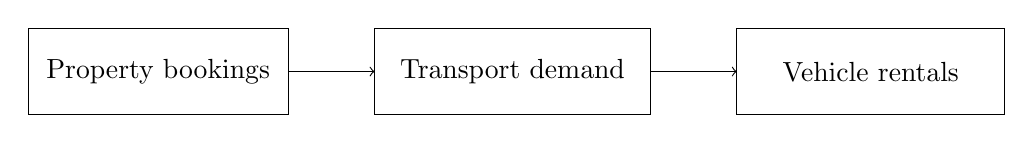
\begin{tikzpicture}
\draw (0,0) rectangle (3.3,1.1);
\draw (4.4,0) rectangle (7.9,1.1);
\draw (9.0,0) rectangle (12.4,1.1);
\node at (1.65,0.55) {Property bookings};
\node at (6.15,0.55) {Transport demand};
\node at (10.7,0.55) {Vehicle rentals};
\draw[->] (3.3,0.55) -- (4.4,0.55);
\draw[->] (7.9,0.55) -- (9.0,0.55);
\end{tikzpicture}
\end{figure}

This is not a redraw of an actual board figure. It is a cleaned statement of the lecture's operating logic.

The fleet size is reported as
\begin{equation}
N_{\text{fleet}} \approx 6,
\end{equation}
and the transcript then gives its most explicit unit economics:
\begin{align}
G_{\text{month,exotic}} &\approx \$8{,}000-\$10{,}000 \quad \text{on some cars},\\
r_{\text{R8}} &\approx \$600-\$700 \text{ per day}.
\end{align}

To see what these figures imply, we may write the standard consistency check
\begin{equation}
G_{\text{month,car}} \approx r_{\text{day}}\,d_{\text{booked}},
\end{equation}
hence
\begin{equation}
d_{\text{booked}} \approx \frac{G_{\text{month,car}}}{r_{\text{day}}}.
\end{equation}

If we insert the quoted ranges only as a rough plausibility test, we get
\begin{equation}
d_{\text{booked}} \approx \frac{\$8{,}000-\$10{,}000}{\$600-\$700}
\approx 11.4-16.7 \text{ booked days/month}.
\end{equation}

This should be read carefully. The lecture does not say that the R8 itself deterministically earns the whole monthly range; it says that some cars do. The estimate is therefore not a derived occupancy law. It is merely a way of seeing why weekend demand is economically meaningful.

\subsection{Question \& Answer}

\paragraph{Question.} How do we get started in exotic car rentals without mistaking the outer layer for the foundation?

\paragraph{Answer.} The lecture answers structurally. First form the LLC. Then learn how the vehicles enter that entity. Then solve the credit and funding problem. Some brands may be more accommodating than others, but income and down payment still matter. Most importantly, the exotic layer works best when it is added to something more fundamental rather than used as the only base.

In compact form,
\begin{equation}
\text{LLC} + \text{credit/funding}
\to
\text{vehicle acquisition}
\to
\text{rental revenue}.
\end{equation}

\begin{remark}
The transcript repeatedly prints ``RA,'' but the surrounding context makes clear that the intended car is the Audi R8. The normalization is safe, though the transcript itself remains noisy.
\end{remark}

\section{Summary}

The lecture begins with spectacle and ends with structure. A million-dollar year, a \$15\text{M}--\$20\text{M} net worth, roughly half a million drawings, nearly forty properties, six cars, and an R8 renting at roughly \$600--\$700 per day: these are the visible outputs. The lecture's deeper work is to show the machinery underneath them.

Across all the interviews, the same small set of rules returns. We scale in stages. We do not lever ignorance. We treat reputation as cumulative. We work through friction rather than waiting for frictionless conditions. We value land through scarcity, carrying cost, and optionality. We let long horizons compound craft. We research before taking the first deal. And when we build a glamorous outer layer, we build it on top of something already cash-flowing.

That is why the lecture holds together. It is not a pile of success stories. It is an argument, assembled interview by interview, that wealth is less a single event than a sequence of learnable operating rules.